\begin{figure}[H]
\centering
\includegraphics[page=6,width=0.33\textwidth]{\FCNCFigures/xTFW/showFake/NOMINAL/reg2mtau1b2jos_vetobtagwp70_highmet/tautaumass.pdf}
\put(-40, 80){\textbf{(a1)}}
\includegraphics[page=6,width=0.33\textwidth]{\FCNCFigures/xTFW/showFake/NOMINAL/reg2mtau1b2jos_vetobtagwp70_highmet/ttvismass.pdf}
\put(-40, 80){\textbf{(a2)}}
\includegraphics[page=6,width=0.33\textwidth]{\FCNCFigures/xTFW/showFake/NOMINAL/reg2mtau1b2jos_vetobtagwp70_highmet/t1mass.pdf}
\put(-60, 80){\textbf{(a3)}}
\\
\includegraphics[page=6,width=0.33\textwidth]{\FCNCFigures/xTFW/showFake/NOMINAL/reg2mtau1b3jos_vetobtagwp70_highmet/tautaumass.pdf}
\put(-40, 80){\textbf{(b1)}}
\includegraphics[page=6,width=0.33\textwidth]{\FCNCFigures/xTFW/showFake/NOMINAL/reg2mtau1b3jos_vetobtagwp70_highmet/ttvismass.pdf}
\put(-40, 80){\textbf{(b2)}}
\includegraphics[page=6,width=0.33\textwidth]{\FCNCFigures/xTFW/showFake/NOMINAL/reg2mtau1b3jos_vetobtagwp70_highmet/drtautau.pdf}
\put(-40, 80){\textbf{(b3)}}
\label{fig:mva_input_hadhad}

\caption{ The BDT input distributions for the background and merged signal in the $t_h\thadhad$-2j (a1-3), $t_h\thadhad$-3j (b1-3) regions of hadronic channel.Only statistical uncertainties are being shown. Underflow and overflow bins are included respectively in the first and last bins. The real tau contributions shown from various MC samples.}% The Kolmogorov Test values for the training and testing BDT distributions are also indicated.
\end{figure}

\begin{figure}[H]
\centering
\includegraphics[page=6,width=0.33\textwidth]{\FCNCFigures/tthML/showFake/faketau/postfit/NOMINAL_fancpaper/reg1l1tau1b2j_os_vetobtagwp70_highmet/x1fit.pdf}
\put(-70, 80){\textbf{(a1)}}
\includegraphics[page=6,width=0.33\textwidth]{\FCNCFigures/tthML/showFake/faketau/postfit/NOMINAL_fancpaper/reg1l1tau1b2j_os_vetobtagwp70_highmet/x2fit.pdf}
\put(-70, 80){\textbf{(a2)}}
\includegraphics[page=6,width=0.33\textwidth]{\FCNCFigures/tthML/showFake/faketau/postfit/NOMINAL_fancpaper/reg1l1tau1b2j_os_vetobtagwp70_highmet/ttvismass.pdf}
\put(-70, 80){\textbf{(a3)}}
\\
\includegraphics[page=6,width=0.33\textwidth]{\FCNCFigures/tthML/showFake/faketau/postfit/NOMINAL_fancpaper/reg1l1tau1b3j_os_vetobtagwp70_highmet/x1fit.pdf}
\put(-70, 80){\textbf{(b1)}}
\includegraphics[page=6,width=0.33\textwidth]{\FCNCFigures/tthML/showFake/faketau/postfit/NOMINAL_fancpaper/reg1l1tau1b3j_os_vetobtagwp70_highmet/x2fit.pdf}
\put(-70, 80){\textbf{(b2)}}
\includegraphics[page=6,width=0.33\textwidth]{\FCNCFigures/tthML/showFake/faketau/postfit/NOMINAL_fancpaper/reg1l1tau1b3j_os_vetobtagwp70_highmet/ttvismass.pdf}
\put(-70, 80){\textbf{(b3)}}
\label{fig:mva_input_lephad}
\caption{ The BDT input distributions for the background and merged signal in the $t_h\tlhad$-2j (a1-3), $t_h\tlhad$-3j (b1-3) regions of leptonic channel.Only statistical uncertainties are being shown. Underflow and overflow bins are included respectively in the first and last bins. The real tau contributions shown from ttbar and other MC including diboson, single top, and V+jets.}% The Kolmogorov Test values for the training and testing BDT distributions are also indicated.
\end{figure}

\begin{figure}[H]
\centering
\includegraphics[page=6,width=0.33\textwidth]{\FCNCFigures/tthML/showFake/faketau/postfit/NOMINAL_fancpaper/reg1l2tau1bnj_os/ttvismass.pdf}
\put(-60, 80){\textbf{(a1)}}
\includegraphics[page=6,width=0.33\textwidth]{\FCNCFigures/tthML/showFake/faketau/postfit/NOMINAL_fancpaper/reg1l2tau1bnj_os/drtautau.pdf}
\put(-40, 80){\textbf{(a2)}}
\includegraphics[page=6,width=0.33\textwidth]{\FCNCFigures/tthML/showFake/faketau/postfit/NOMINAL_fancpaper/reg1l2tau1bnj_os/t2vismass.pdf}
\put(-60, 80){\textbf{(a3)}}
\\
\includegraphics[page=6,width=0.33\textwidth]{\FCNCFigures/tthML/showFake/faketau/postfit/NOMINAL_fancpaper/reg1l1tau1b1j_ss_vetobtagwp70_highmet/tau_pt_0.pdf}
\put(-60, 80){\textbf{(b1)}}
\includegraphics[page=6,width=0.33\textwidth]{\FCNCFigures/tthML/showFake/faketau/postfit/NOMINAL_fancpaper/reg1l1tau1b1j_ss_vetobtagwp70_highmet/drlb.pdf}
\put(-40, 80){\textbf{(b2)}}
\includegraphics[page=6,width=0.33\textwidth]{\FCNCFigures/tthML/showFake/faketau/postfit/NOMINAL_fancpaper/reg1l1tau1b1j_ss_vetobtagwp70_highmet/drtaujmin.pdf}
\put(-80, 80){\textbf{(b3)}}
\\
\includegraphics[page=6,width=0.33\textwidth]{\FCNCFigures/tthML/showFake/faketau/postfit/NOMINAL_fancpaper/reg1l1tau1b2j_ss_vetobtagwp70_highmet/tau_pt_0.pdf}
\put(-60, 80){\textbf{(c1)}}
\includegraphics[page=6,width=0.33\textwidth]{\FCNCFigures/tthML/showFake/faketau/postfit/NOMINAL_fancpaper/reg1l1tau1b2j_ss_vetobtagwp70_highmet/drlb.pdf}
\put(-40, 80){\textbf{(c2)}}
\includegraphics[page=6,width=0.33\textwidth]{\FCNCFigures/tthML/showFake/faketau/postfit/NOMINAL_fancpaper/reg1l1tau1b2j_ss_vetobtagwp70_highmet/x1fit.pdf}
\put(-60, 80){\textbf{(c3)}}
\\
\caption{ The BDT input distributions for the background and merged signal in the $t_l\thadhad$ (a1-3), $t_l\thad$-1j (b1-3), $t_l\thadhad$-2j (c1-3) regions of leptonic channel.Only statistical uncertainties are being shown. Underflow and overflow bins are included respectively in the first and last bins. The real tau contributions shown from ttbar and other MC including diboson, single top, and V+jets.}% The Kolmogorov Test values for the training and testing BDT distributions are also indicated.
\label{fig:mva_input_lhadhad}
\end{figure}